\documentclass[apj]{emulateapj}

%Specify packages
\usepackage{amsmath}
\usepackage{tikz}
\usetikzlibrary{shapes.geometric, arrows}
\usepackage[tight]{subfigure}
\usepackage[breaklinks,colorlinks,citecolor=blue]{hyperref}
\usepackage[all]{hypcap}
\usepackage[utf8]{inputenc} %force unicode in bibtex
\usepackage{enumitem}
%use for editing/highlighting
\usepackage{color,soul}


%Define new commands as needed
\newcommand{\ang}{\AA~}
\defcitealias{cargill_hot_2016}{Paper I}
\renewcommand{\sectionautorefname}{Section}
\renewcommand{\subsectionautorefname}{Subsection}
%Set options for list spacing
\setenumerate{noitemsep}
%Set tikz options
\tikzstyle{box} = [rectangle, rounded corners, text centered, draw=black]
\tikzstyle{ghost} = [rectangle, rounded corners, text centered, draw=white]
\tikzstyle{arrow} = [thick, ->, >=stealth]

\begin{document}
	%Frontmatter
	\title{``Hot'' Non-flaring Plasma in Active Regions II. Impacts of Two-fluid Effects on Emission from Impulsively Heated Loops}
	\author{W. T. Barnes}
	\author{S. J. Bradshaw}
	\affil{Department of Physics \& Astronomy, Rice University, Houston, TX 77251-1892}
	\email{will.t.barnes@rice.edu}
	\author{P. J. Cargill}
	\affil{Space and Atmospheric Physics, The Blackett Laboratory, Imperial College, London SW7 2BW}
	\affil{School of Mathematics and Statistics, University of St. Andrews, St. Andrews, Scotland KY16 9SS}
	%Abstract
	\begin{abstract}
		Faint, high-temperature emission in active region cores has long been predicted as a signature of nanoflare heating. However, the detection of such emission has proved difficult due to a combination of the efficiency of thermal conduction, non-equilibrium ionization, and inadequate instrument sensitivity. This second paper in our series on hot non-flaring plasma in active regions aims to show how the assumption of electron-ion equilibrium leads to misleading conclusions regarding the hot emission. We have used an efficient two-fluid hydrodynamic model to carry out a parameter exploration in preferentially heated species, heating event frequency, and the power-law index determining the distribution of event energies. By computing the emission measure distributions and calculating their ``hotward'' slopes, we have concluded that the assumption of electron-ion equilibrium leads to an understimate of the amount of hot plasma at intermediate and high heating frequencies. Additionally, we find that, while emission due to separate electron and ion heating differs greatly hotward of the peak, the respective coolward emission measure slopes are similar such that a distinction between the heating of one species over another based on this criteria alone is not possible. 
	\end{abstract}
	%Body
	\section{Introduction}
	\label{sec:intro}
	%
	\par The nanoflare heating model, first proposed by \citet{parker_nanoflares_1988}, has become one of the most favored and contentious coronal heating models \citep{cargill_implications_1994,cargill_nanoflare_2004,klimchuk_solving_2006}. While many theoretical efforts \citep[e.g.][]{bradshaw_diagnosing_2012,reep_diagnosing_2013,cargill_active_2014} have shown the feasability of nanoflares, the idea has long suffered from a lack observational evidence. The term \textit{nanoflare} has now become synonomous with impulsive heating in the energy range $10^{24}-10^{27}$ erg, with no specific assumption as to what underlying physical mechanism is responsible. However, while we ascribe no particular source (e.g. waves versus reconnection) to this bursty energy release, its origin is almost certainly magnetic.
	%
	\par \citet{cargill_implications_1994} and \citet{cargill_nanoflare_2004} have predicted that emission measure distributions resulting from nanoflare models should be wide and have a faint, high-temperature (8-10 MK) component and thus a steep hotward slope, the so-called ``smoking gun'' of nanoflare heating. Unfortunately, observing this high-temperature emission is difficult and in some cases impossible. The reason for this difficulty is twofold. First, thermal conduction is a very efficient cooling mechanism at high temperatures and large spatial temperature gradients. When a loop is heated impulsively, its temperature rises quickly while the increase in density lags behind. By the time the density has increased sufficiently (due to chromospheric evaporation brought about by the response of the transition region to the strong downward coronal heat flux) to allow for an appreciable amount of emission (recalling $\mathrm{EM}\propto n^2$), thermal conduction has cooled the loop far below its initial hot temperature, making a direct detection of $\sim10$ MK plasma very difficult. 
	%
	\par The second reason for this difficulty is non-equilibrium ionization. It is usually assumed that the observed emission lines, because of their known formation temperatures, are a direct indicator of the plasma temperature. However, if the heating timescale is shorter than the ionization equilibration timescale, the time it takes for the ion population to settle into the assumed charge state, an equilibrium assumption can lead to a misdiagnosis of the plasma temperature. This makes signatures of hot, nanoflare-heated plasma especially difficult to detect if the high temperatures persist for less than the ionization timescale \citep{bradshaw_explosive_2006,bradshaw_what_2011,reale_nonequilibrium_2008}.
	%
	\par Despite these difficulties, various attempts have been made to observe this faint high-temperature emission. Using the broadband X-Ray Telescope (XRT) \citep{golub_x-ray_2007} on board the \textit{Hinode} spacecraft \citep{kosugi_hinode_2007}, \citet{schmelz_hinode_2009} and \citet{reale_evidence_2009} show a faint hot component in the reconstructed $\mathrm{DEM}$ curves. However, since the channels on such broadband instruments can often be polluted by low-temperature emission, the reliability of such measurements depends on the filtering technique used. Additionally, \citet{winebarger_defining_2012} showed that combinations of measurements from XRT and the Extreme-ultraviolet Imaging Spectrometer (EIS) \citep{culhane_euv_2007}, also on  \textit{Hinode}, leave a ``blind spot'' in the $\mathrm{EM}-T$ space conincident with the range where evidence for nanoflare heating is likely to be found. 
	%
	\par Unambiguous observational evidence of nanoflare heating must come from pure spectroscopic measurements \citep[see][]{brosius_pervasive_2014}. Additionally, new instruments with higher spatial and temporal resolution, such as \textit{IRIS} \citep{de_pontieu_interface_2014} and the \textit{Hi-C} sounding rocket \citep{cirtain_energy_2013} have provided encouraging results for impulsive heating \citep{testa_observing_2013,testa_evidence_2014}. Future missions like the Marshall Grazing Incidence X-ray Spectrometer (MaGIXS) \citep{kobayashi_marshall_2011,winebarger_new_2014}, with a wavelength range of 6-24 \ang and a temperature range of $6.2<\log{T}<7.2$, aim to probe this previously poorly-resolved portion of the coronal spectrum in hopes of better quantifying the presence of faint, high-temperature plasma.
	%
	\par One strategy for constraining the nanoflare model is analysis of modelled and observed emission measure distributions for signatures of impulsive heating in active region cores. As with cool emission, hot emission is also often characterized by a power-law relation of the form $\mathrm{EM}\propto T^{-b}$. Typically, this power-law fit to the emission measure is done ``hotward'' of the peak, usually in the range $6.6\lesssim\log{T}\lesssim7.2$. However, measured values of these hotward slopes are poorly constrained due to both the magnitude of emission and the lack of available spectroscopic data in this temperature range. \citet{warren_systematic_2012}, using spectral measurements from EIS, provided hotward fits for $\mathrm{EM}$ reconstructions for a large number of active regions. All measured slopes fell in the range $6.1<b<10.3$, with large uncertainties on each hotward fit.
	%
	\par An often overlooked consequence of impulsive heating in the corona is electron-ion non-equilibrium. In a fully-ionized hydrogen plasma like the solar corona, interactions between electrons and ions are governed by binary Coulomb collisions. For $n\sim10^8~\mathrm{cm}^{-3}$ and $T\sim10^7~\mathrm{K}$, parameters typical of nanoflare heating, the collisional timescale, $\tau_{ei}=1/\nu_{ei}$, where $\nu_{ei}$ is the Coulomb collision frequency (see \autoref{eq:col_freq}) can be estimated as $\tau_{ei}\approx8000$ s. Thus, any heating that occurs on a timescale less than 8000 s, such as a nanoflare with a durration of $\tau_H\le100$ s, will result in electron-ion non-equilibrium. Chromospheric evaporation, the response from the transition region to the strong coronal heat flux, does lead to an increase in $n$ and thus a decrease in $\tau_{ei}$. However, we maintain that during this initial phase of impulsive heating, $\tau_{ei}\gg\tau_H$ still holds, with 8000 s being an approximate upper bound on $\tau_{ei}$. 
	%
	\par Additionally, while it is often assumed that the electrons are the direct recipients of the prescribed heating function, the degree to which the ions or electrons are preferentially heated in the solar corona is unknown. Thus, it is possible that the ions are preferentially heated, for instance, through ion-cyclotron wave resonances \citep{markovskii_intermittent_2004}. Ion cyclotron waves are excited by plasma instabilities in the lower corona. These waves then propagate upwards through the coronal plasma and wave particle interactions can occur for those ions whose gyrofrequencies have a resonance with the ion-cyclotron wave. Additionally, there is also evidence for ion heating via reconnection, both in laboratory plasmas and in particle-in-cell simulations \citep{ono_ion_1996,yoo_bulk_2014,drake_onset_2014}. Thus, ion heating in the solar corona should not be discounted as a possibility.
	%
	\par In our first paper, \citet{cargill_hot_2016} \citepalias[hereafter]{cargill_hot_2016}, we studied the effect of pulse duration, flux limiting, and non-equilibrium ionization on hot emission from single nanoflares and nanoflare trains. In this second paper in our series on hot emission in active region cores, we will use an efficient two-fluid hydrodynamic model to explore the effect of electron and ion heating on nanoflare-heated loops. In particular, we will look at how the hot emission is affected by heating preferentially one species or the other as well as how this hot emission can vary with heating frequency and the power-law index that determines the event energy distribution. 
	\par\autoref{sec:methods} discusses the numerical model we have used to conduct this study and the parameter space we have investigated. \autoref{sec:results} shows the resulting emission measure curves and slopes for the electron and ion heating cases as well as the equivalent single-fluid cases. In \autoref{sec:discussion}, we discuss the implications of two-fluid effects in the context of hot and cool emission measure slopes and the nanoflare heating model. Finally, \autoref{sec:conclusions} provides some concluding comments on our findings.
	%%
	\section{Methodology}
	\label{sec:methods}
	%
	\subsection{Numerical Model}
	\label{subsec:numerics}
	%
	\par 1D hydrodynamic models are excellent tools for computing field-aligned quantities in coronal loops. However, because of the small cell sizes needed to resolve the transition region and consequently small timesteps demanded by thermal conduction, the use of such models in large parameter sweeps is made impractical by long computational runtimes \citep{bradshaw_influence_2013}. Thus, in our numerical study, we use a modified form of the popular 0D enthalpy-based thermal evolution of loops (EBTEL) model \citep{klimchuk_highly_2008,cargill_enthalpy-based_2012,cargill_enthalpy-based_2012-1,cargill_modelling_2015}. This model, which has been successfully benchmarked against the 1D hydrodynamic HYDRAD code of \citet{bradshaw_influence_2013}, computes time-dependent spatially-averaged loop quantities with very low computational overhead and as such is ideal for large parameter space investigations.
	%
	\par We have modified the usual EBTEL equations \citep[see][]{cargill_enthalpy-based_2012} to treat the evolution of the electron and ion populations separately while maintaining the assumption of quasi-neutrality, $n_e=n_i=n$. This amounts to computing spatial averages of the two-fluid hydrodynamic equations over both the transition region and corona. We will reserve a full discussion of this modified EBTEL model for a future paper. The relevant equations can be found in \autoref{appendix}.  
	%%
	\subsection{Parameter Space}
	\label{subsec:params}
	%
	\par We define our heating function in terms of a series of discrete heating events plus a static background heating rate to ensure that the loop does not drop to unphysically low temperatures and densities between events. All events are modeled as triangular pulses of fixed duration $\tau_H=100$ s. Thus, for loop half-length $L$ and cross-sectional area $A$, the total energy per event is $Q_i=LAH_i\tau_H/2$, where $H_i$ is the heating rate amplitude of event $i$. Each run will consist of $N$ heating events, each with peak amplitude $H_i$, and a steady background value of $H_b=3.4\times10^{-6}$ erg cm$^{-3}$ s$^{-1}$.
	%
	\begin{figure}
		\centering
			\begin{tikzpicture}[node distance=2cm]
		%Draw the nodes
		\node (species) [ghost] {$\Sigma=\left\{
		\begin{array}{l}
			\mathrm{electron} \\
			\mathrm{ion} \\
			\mathrm{single}
		\end{array}
		\right.$};
		\node (ghost_ph) [ghost, below of=species] {};
		\node (alpha_pl) [ghost, left of=ghost_ph] {$\alpha=\left\{
		\begin{array}{l}
			-1.5 \\
			-2.0 \\
			-2.5
		\end{array}
		\right.$};
		\node (alpha_uni) [ghost, right of=ghost_ph] {uniform};
		\node (ghost_beta) [ghost, below of=alpha_pl]{};
		\node (beta_1) [ghost, right of=ghost_beta] {$\beta=1$};
		\node (beta_0) [ghost, left of=ghost_beta] {$\beta=0$};
		%Draw the arrows
		\draw [arrow] (species) -- (alpha_pl);
		\draw [arrow] (species) -- (alpha_uni);
		\draw [arrow] (alpha_pl) -- (beta_0);
		\draw [arrow] (alpha_pl) -- (beta_1);
		%\draw [arrow] (alpha_pl) -- (beta_2);	
	\end{tikzpicture}
		\caption{Total Parameter space covered. $\Sigma$ indicates the species that is heated, where ``single'' indicates a single-fluid model. $\alpha$ is the power-law index and $\beta$ indicates the scaling in the relationship $Q\propto T_N^{\beta}$, where $\beta=0$ corresponds to the case where $T_N$ and the event energy are independent. Note that $(3~\alpha~\mathrm{values})\times(3~\beta~\mathrm{values})+\mathrm{uniform~heating}=$ 10 different types of heating functions.}
		\label{fig:parameter_space}
	\end{figure}
	%
	\par Observations have suggested that loops in active region cores are maintained at an equilibrium temperature of $T_{peak}\approx4$ MK \citep{warren_constraints_2011,warren_systematic_2012}. The corresponding heating rate can be estimated using coronal hydrostatics. Neglecting the radiative loss term and letting $dF_C/ds\approx\kappa_0T_{peak}^{7/2}/L^2$, $E_{H,eq}$ can be estimated as 
	\begin{equation}
		\label{eq:heating_rate_est}
		E_{H,eq} \approx \frac{\kappa_0T_{peak}^{7/2}}{L^2},
	\end{equation}
	where $\kappa_0\approx10^{-6}~\mathrm{erg}~\mathrm{K}^{-7/2}~\mathrm{cm}^{-1}~\mathrm{s}^{-1}$. $E_{H,eq}$ can be interpreted as a time-averaged volumetric heating rate. Thus, to maintain an emission measure peaked about $T_{peak}$, for triangular pulses, the individual heating rates are constrained by 
	\begin{equation}
		\label{eq:heating_rate_constraint}
		E_{H,eq} = \frac{1}{T}\sum_{i=1}^N\int_{t_i}^{t_i+\tau_H}\mathrm{d}t~h_i(t) = \frac{\tau_H}{2T}\sum_{i=1}^NH_i.
	\end{equation}
	where $T$ is the total simulation time. Note that if $H_i=H_0$ for all $i$, the uniform heating amplitude $H_0$ is just $H_0=2TE_{H,eq}/N\tau_H$. Thus, for $L=40$ Mm, $A=10^{14}$ cm$^2$, the total amount of energy injected into the loop by one heating event for a loop heated by $N=20$ nanoflares in $T=80000$ s is $Q=LATE_{H,eq}/N\approx1.3\times10^{25}$ erg, consistent with the energy budget of the Parker nanoflare model. 
	%
	\par Determining the heating frequency in active region cores will help to place constraints on the source(s) of heat in the corona. We define the heating frequency in terms of the waiting time, $T_N$, between successive heating events. Following \citet{cargill_active_2014}, the range of waiting times is $250\le T_N\le5000$ s in increments of 250 s, for a total of 20 different possible heating frequencies. Additionally, $T_N$ can be written as $T_N=(T-N\tau_H)/N$, where we fix $T=80000$ s. Note that because $T$ and $\tau_H$ are fixed, as $T_N$ increases, $N$ decreases. Correspondingly, $Q_i$, the energy injected per event, increases according to \autoref{eq:heating_rate_constraint} such that the total energy injected per run is constant, regardless of $T_N$.
	%
	\begin{figure}
		\centering
		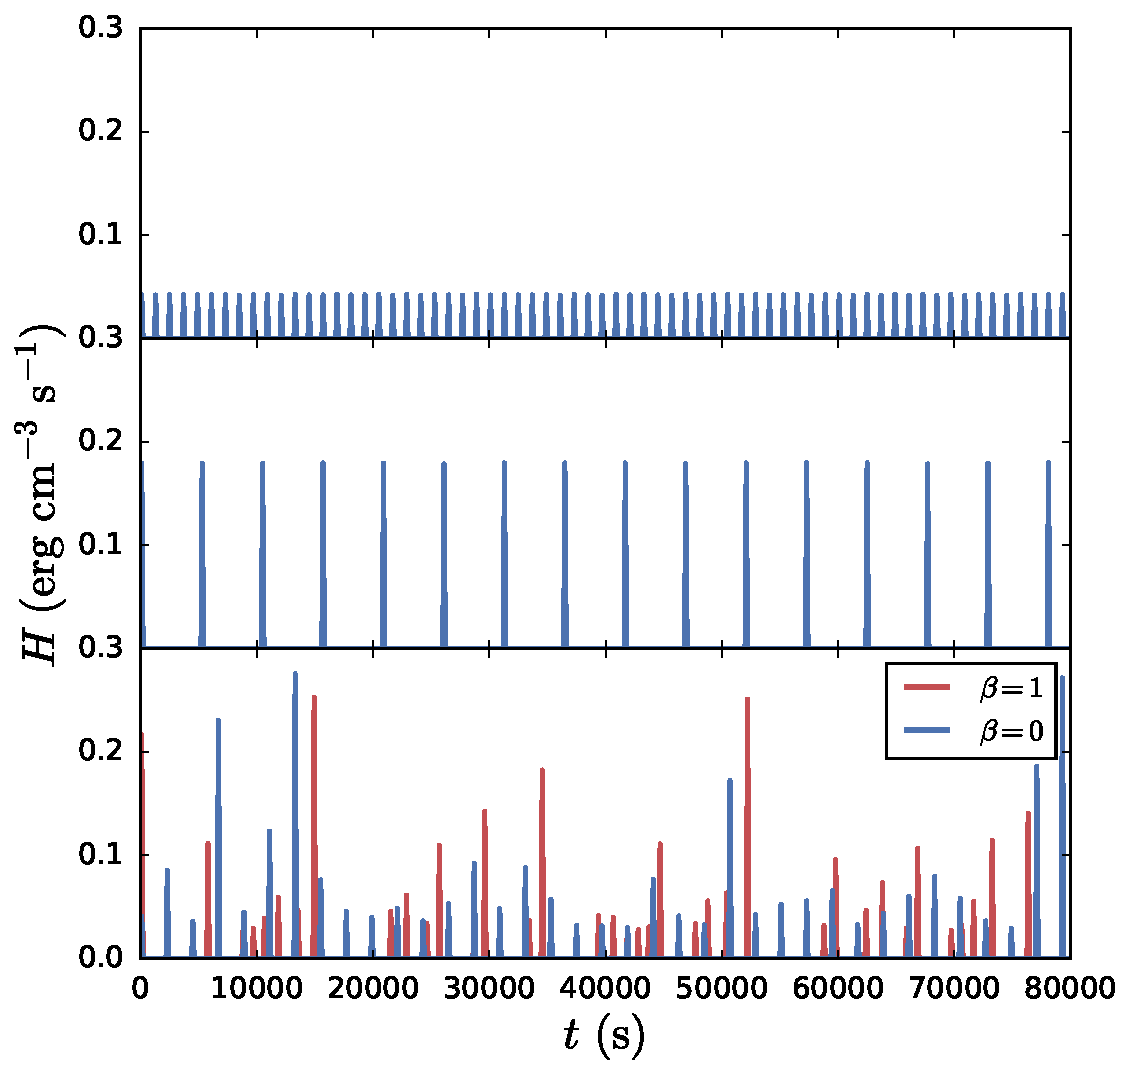
\includegraphics[width=\columnwidth]{figures/heating_functions.pdf}
		\caption{\textbf{Top left}: uniform heating amplitudes for $T_N=1000$ s; \textbf{Top right:} uniform heating amplitudes for $T_N=5000$ s; \textbf{Bottom left:} power-law distributed heating amplitudes for $\alpha=-1.5$, $T_N=2000$ s; \textbf{Bottom right:} power-law distributed amplitudes for $\alpha=-1.5$ where the wait times depend on the event energies and the mean wait time for both values of $\beta$ is $\langle T_N\rangle=2000$ s.}
		\label{fig:heating_funcs}
	\end{figure}
	%
	\par We compute the peak heating rate per event in two different ways: 1) the heating rate is uniform such that $H_i=H_0$ for all $i$ and 2) $H_i$ is chosen from a power-law distribution with index $\alpha$ where $\alpha=-1.5,-2.0,$ or $-2.5$. For the second case, it should be noted that, when $T_N\approx5000$ s, $N\sim20$ events, meaning a single run does not accurately represent the distribution of index $\alpha$. Thus, a sufficiently large number of runs, $N_{R}$, are computed for each $T_N$ to ensure that the total number of events is $N_{tot}=N\times N_{R}\sim10^4$ such that the distribution is well-represented. \autoref{fig:parameter_space} shows the parameter space we will explore. For each set of parameters and waiting time $T_N$, we compute the resulting emission measure distribution for $N$ events in a period $T$. This procedure is repeated $N_R$ times until $N\times N_R\sim10^4$ is satisfied.
	%
	\par According to the nanoflare heating model of \citet{parker_nanoflares_1988}, turbulent loop footpoint motions twist and stress the field, leading to a buildup and subsequent release of energy. Following \citet{cargill_active_2014}, we let $Q_i\propto T_{N,i}^{\beta}$, where $Q_i,T_{N,i}$ are the total energy and waiting time following event $i$, respectively, and $\beta=1,2$ such that the event energy scales either linearly or quadratically with the waiting time. The reasoning for such an expression is as follows. Bursty, nanoflare heating is thought to arise from the stressing and subsequent relaxation of the coronal field. If a sufficient amount of time has elapsed since the last energy release event, the field will have had enough time to ``wind up'' such that the subsequent energy release is large. Conversely, if only a small amount of time has elapsed since the last event, the field will have not had time to become as stressed, resulting in a lower energy event. Thus, this scaling provides a way to incorporate a more physically motivated heating function into a hydrodynamic model which cannot self-consistently determine the heat input based on the evolving magnetic field. \autoref{fig:heating_funcs} shows the various heating functions used for several example $T_N$ values.
	%
	\subsection{Emission Measure Distributions}
	\label{subsec:em_dist}
	%
	\par In our 0D model, the emission measure is calculated using the familiar expression $\mathrm{EM}=n^2(2L)$, where $L$ is the loop half-length. We consider a temperature range of $4.0\le\log{T}\le8.5$ with bin sizes of $\Delta\log{T}=0.01$. At each iteration $i$, the coronal temperature range $[T_0,T_a]$ is calculated from $\bar{T}_e$ (see \autoref{appendix}). For each bin that falls within $[T_0,T_a]$, $\bar{n}_i^2(2L)$ is added to that bin, where $\bar{n}_i$ is the spatially-averaged number density at iteration $i$. The emission measure in each bin is then averaged over the entire simulation period. We do not attempt to apply an advanced forward modeling treatment here and instead reserve such an approach for a future paper. Thus, effects due to insufficient instrument sensitivity or non-equilibrium ionization are not included.
	%
	\section{Results}
	\label{sec:results}
	%
	\par For each species, type of power-law heating function, and waiting time $T_N$, $N_{R}$ emission measure curves are calculated. Because drawing event amplitudes from a power-law distribution introduces random fluctuations into our model, we must be sure to account for the full range of effects due to the distribution. This is especially true in the low-frequency regime, when $T_N\ge\tau_{cool}$, the cooling timescale, and there are fewer events per run. In this case, one or two especially strong heating events can lead to an extremely enhanced hotward emission measure; conversely, a run with only small events will lead to a diminished hotward slope. Thus, the mean $\mathrm{EM}$ curve of each set of $N_{R}$ runs can be said to reasonably represent the expected hot emission for a given $T_N$.
	%
	\par To characterize the emission measure, we compute the slopes on both the cool and hot sides of the peak. To be consistent with past observational and computational studies of cool emission \citep[see][and references therein]{bradshaw_diagnosing_2012}, we fit the cool slope on the interval $6.0\le\log{T}\le6.6$. Contrastingly, past studies of hot emission are less abundant; thus, the ``hot'' region where $\mathrm{EM}$ is known to follow a power-law is far less constrained. In order to best describe the steepness of the emission measure hotward of the peak, we choose to fit $\mathrm{EM}$ between the temperatures at which the emission measure is $99\%$ and $92\%$ of the peak value. We have no physical reason for choosing these particular bounds, but note that on this interval, the mean hotward emission is reasonably well described by a linear relationship. Fitting too close to the wide peak leads to misleadingly shallow slopes while fitting too close to the steep drop near $\log{T}\sim7.5$ results in steep slopes not particularly representative of the hotward emission. We perform the fit using the Levenberg-Marquardt algorithm for least-squares curve fitting as implemented in the SciPy scientific Python package \citep{van_der_walt_numpy_2011}.
	%
	\subsection{Separate Electron and Ion Heating}
	\label{subsec:electron_ion_heating}
	%
	\begin{figure*}
		\centering
		\begin{minipage}[c]{0.49\textwidth}
			\subfigure{%
			\includegraphics[width=\columnwidth]{figures/{ebtel_L40.0_tpulse100.0_alpha2.5-b1.0_electron_heating_dem}.pdf}
			\label{fig:el_em_curves}}
		\end{minipage}
		%
		\begin{minipage}[c]{0.49\textwidth}
			\subfigure{%
			\includegraphics[width=\columnwidth]{figures/{ebtel_L40.0_tpulse100.0_alpha2.5-b1.0_electron_heating_hs_compare}.pdf}
			\label{fig:el_em_slopes}}
			\subfigure{%
			\includegraphics[width=\columnwidth]{figures/{ebtel_L40.0_tpulse100.0_alpha2.5-b1.0_electron_heating_dem_derivs}.pdf}
			\label{fig:el_em_derivs}}
		\end{minipage}
		\caption{$\alpha=-2.5,~\beta=1,~L=40$ Mm, electron heating. \textbf{Left:} $\log{\mathrm{EM}}$ as a function of $\log{T}$ for all values of $T_N$. There is an artificial spacing of $\Delta\log{\mathrm{EM}}=0.2$ between each curve. The bold blue (red) lines on either side of the peak show the linear fit to the cool (hot) emission. \textbf{Top right:} Average slopes from power-law fits to all $N_{R}$ curves as a function of $T_N$. The error bars indicate one standard deviation from the distribution of $N_{R}$ fits. In the case of hot slopes, the absolute value is shown. The dashed, solid, and dot-dashed reference lines are placed at 2, 3, and 5 respectively. \textbf{Bottom right:} Derivative of $\log{\mathrm{EM}}$ with respect to $\log{T}$. The dotted reference lines are placed at -5.5, -2.5, 2, and 3. The legend is the same as the left panel.}
		\label{fig:el_em}
	\end{figure*}
	%
	\begin{figure*}
		\centering
		\begin{minipage}[c]{0.49\textwidth}
			\subfigure{%
			\includegraphics[width=\columnwidth]{figures/{ebtel_L40.0_tpulse100.0_alpha2.5-b1.0_ion_heating_dem}.pdf}
			\label{fig:ion_em_curves}}
		\end{minipage}
		%
		\begin{minipage}[c]{0.49\textwidth}
			\subfigure{%
			\includegraphics[width=\columnwidth]{figures/{ebtel_L40.0_tpulse100.0_alpha2.5-b1.0_ion_heating_hs_compare}.pdf}
			\label{fig:ion_em_slopes}}
			\subfigure{%
			\includegraphics[width=\columnwidth]{figures/{ebtel_L40.0_tpulse100.0_alpha2.5-b1.0_ion_heating_dem_derivs}.pdf}
			\label{fig:ion_em_derivs}}
		\end{minipage}
		\caption{Same as \autoref{fig:el_em}, but for the case in which all of the heating is given to the ions.}
		\label{fig:ion_em}
	\end{figure*}
	%
	\par \autoref{fig:el_em} and \autoref{fig:ion_em} show the results of our emission measure study for the two distinct cases where only the electrons are heated and only the ions are heated with $\alpha=-2.5,b=1$ for a loop half-length of $40$ Mm, consistent with \citetalias{cargill_hot_2016}. The panels on the left show the mean $\mathrm{EM}$ for all $T_N$, where the average is taken over all $N_{R}$ runs. There is an artifical spacing of $\Delta\log{\mathrm{EM}}=0.2$ between each curve so that they can be easily distinguished from each other. The blue (red) lines indicate the cool (hot) power-law fits, where the slopes of the lines are the averages taken over all $N_{R}$ runs. We note that $\mathrm{EM}$, for all $T_N$, peaks at approximately 4 MK ($10^{6.6}$ K), consistent with the constraints laid out in \autoref{subsec:params}. The top right panels show these average slope values as a function of $T_N$. The error bars indicate one standard deviation as calculated from the distribution of all $N_{R}$ runs.
	%
	\par Lastly, the bottom right panels show the first derivative as a function of temperature, $d\log{\mathrm{EM}}/d\log{T}$, computed using central differences. The color scheme and line styles correspond to the emission mesure curves in the left panel. As in \citetalias{cargill_hot_2016}, we compute the derivative in an effort to better assess at what temperatures the emission measure is not well described by a power-law.
	%
	\par We first briefly consider the calculated cool emission measure slopes. Looking at the top right panels of \autoref{fig:el_em} and \autoref{fig:ion_em}, we note that in the cases of electron and ion heating, the cool emission measure slopes are consistent with both observational and modelling studies of cool emission in active region cores, having values that fall within the range $2\le a\le5$ \citep[and references therein]{bradshaw_diagnosing_2012}. Furthermore, the cool slopes computed using our new modified EBTEL model, with a heating function of the form $Q\propto T_N^{\beta}$, are consistent with those values reported in \citet{cargill_active_2014} and show a dependence on the waiting time $T_N$.  
	%
	\par Additionally, looking at the bottom right panels of \autoref{fig:el_em} and \autoref{fig:ion_em}, we see that, within the range $6.0\le\log{T}\le6.6$, a linear approximation of $\mathrm{EM}$ on a log-log scale is reasonable, where $2\lesssim d\log{\mathrm{EM}/d\log{T}}\lesssim3$. Comparing the cases of electron and ion heating for both the cool slopes and $d\log{\mathrm{EM}/d\log{T}}$ on $6.0\le\log{T}\le6.6$, there are no substantial differences for all values of $T_N$ considered.
	%
	\par This is not the case for the hot emission measure. Looking first at the case of electron heating in \autoref{fig:el_em}, we note that there is a pronounced ``hot shoulder'' in the emission measure (left panel) just above $10^7$ K for $T_N\gtrsim2000$ s. This feature is even more evident when looking at the derivative of $\mathrm{EM}$ in the bottom right panel of \autoref{fig:el_em}. The peak between $10^7$ and $10^{7.5}$ K shows how the $\mathrm{EM}$ flattens out around $10^7$ K, indicating an enhanced hot emission measure. Considering the large range of values of $d\log{\mathrm{EM}}/d\log{T}$ on the interval over which the fit was performed, we acknowledge that a single power-law is not a good description of the hot emission measure in the case of electron heating.
	%
	\par Contrastingly, we have not calculated the hot emission measure slopes for the case of ion heating. Looking at the left panel of \autoref{fig:ion_em}, for $T_N\gtrsim1000$ s, the $\mathrm{EM}$ peak is wide with a steep drop near $10^7$ K. There is no substantial emission measure component above $10^7$ K and, consequently, no hot shoulder as in the electron heating case. Applying the fitting procedure outlined above to the hot emission in the case of ion heating yields meaningful results for only a few short $T_N$. Thus, as in the case of electron heating, the resulting hot emission measure from ion heating is not well described by a power-law. The lower right panel of \autoref{fig:ion_em} further highlights this by showing that around $10^7$ K, $d\log{\mathrm{EM}}/d\log{T}\to-\infty$.
	%
	\subsection{Single-fluid}
	\label{subsec:single_heating}
	%
	\par \autoref{fig:single_em} shows the same results as \autoref{fig:el_em} and \autoref{fig:ion_em}, but for the single-fluid case in which electron-ion equilibrium is assumed at all times. To compute these $\mathrm{EM}$ curves, we have used the original, single-fluid EBTEL model as described in \citet{klimchuk_highly_2008} and \citet{cargill_enthalpy-based_2012}. The equivalent parameter space that was investigated with the modified two-fluid EBTEL model is explored with the single-fluid EBTEL code as well.
	%
	\par We compute the hot and cool emission measure slopes in the same manner as the electron and ion heating cases. We first note that the cool emission measure slopes are comparable to those in both the electron and ion heating cases. In particular, we find $2\lesssim a\lesssim5$ for all values of $T_N$ as expected. Again, we confirm the validity of our linear fit to the cool emission by computing the derivative $d\log{\mathrm{EM}}/d\log{T}$ in the lower right panel of \autoref{fig:single_em}. For $T_N\gtrsim2000$ s, the slope is bounded between 2 and 3 on the interval $6.0\le\log{T}\le6.6$. 
	%
	\par The hot emission measure in the single-fluid case differs significantly from the two-fluid case. In contrast to the electron heating case in \autoref{fig:el_em}, the $\mathrm{EM}$ curves in the left panel of \autoref{fig:single_em} show no hot shoulder. This is further confirmed by the lower right panel; the derivative, in contrast to the electron heating case, shows no peak near $10^7$ K. For low $T_N$, $d\log{\mathrm{EM}}/d\log{T}$ is monotonically decreasing for $\log{T}\gtrsim6.6$. For $T_N\ge3000$ s, $d\log{\mathrm{EM}}/d\log{T}$ is relatively flat for $\log{T}\ge7.0$, indicating that a linear fit is a good description for the hot emission in this region. This is confirmed by noting the agreement between the fit lines and the $\mathrm{EM}$ curves in the left panel.
	%
	\par Comparing the top right panels of \autoref{fig:single_em} and \autoref{fig:el_em} further highlights the enhanced hot emission in the electron case. For high $T_N$, the hot emission slopes in the electron case converge to a value just above 3; for the single-fluid case, the hot slopes converge to approximately 4.5. Thus, while a single power-law is not a good descriptor of the hot emission in the case of electron heating, the slope still captures the enhanced hot shoulder relative to the weaker hot emission of the single-fluid case. Additionally, comparing the single-fluid case to the ion heating case in \autoref{fig:ion_em}, it is obvious that the single-fluid case shows a great deal more hot emission as the $\mathrm{EM}$ curves in the left panel of \autoref{fig:single_em} extend well above $10^7$ K while those in the left panel of \autoref{fig:ion_em} show a steep cutoff at temperatures just above the peak.
	%
	\begin{figure*}
		\centering
		\begin{minipage}[c]{0.49\textwidth}
			\subfigure{%
			\includegraphics[width=\columnwidth]{figures/{ebtel_L40.0_tpulse100.0_alpha2.5-b1.0_single_heating_dem}.pdf}
			\label{fig:single_em_curves}}
		\end{minipage}
		%
		\begin{minipage}[c]{0.49\textwidth}
			\subfigure{%
			\includegraphics[width=\columnwidth]{figures/{ebtel_L40.0_tpulse100.0_alpha2.5-b1.0_single_heating_hs_compare}.pdf}
			\label{fig:single_em_slopes}}
			\subfigure{%
			\includegraphics[width=\columnwidth]{figures/{ebtel_L40.0_tpulse100.0_alpha2.5-b1.0_single_heating_dem_derivs}.pdf}
			\label{fig:single_em_derivs}}
		\end{minipage}
		\caption{Same as \autoref{fig:el_em}, but for the single-fluid case in which electron-ion equilibrium is assumed.}
		\label{fig:single_em}
	\end{figure*}
	%
	\subsection{Full Parameter Space Comparison}
	\label{subsec:all_params}
	%
	\begin{figure*}
		\centering
		\begin{minipage}[c]{0.49\textwidth}
			\subfigure{%
			\includegraphics[width=\columnwidth]{figures/{el_cool_alpha_histo}.pdf}
			\label{fig:el_cool_alpha_histo}}
			\subfigure{%
			\includegraphics[width=\columnwidth]{figures/{el_hot_tn_histo}.pdf}
			\label{fig:el_hot_tn_histo}}
		\end{minipage}
		\begin{minipage}[c]{0.49\textwidth}
			\subfigure{%
			\includegraphics[width=\columnwidth]{figures/{ion_cool_alpha_histo}.pdf}
			\label{fig:ion_cool_alpha_histo}}
			\subfigure{%
			\includegraphics[width=\columnwidth]{figures/{single_hot_tn_histo}.pdf}
			\label{fig:single_cool_tn_histo}}
		\end{minipage}
			\caption{Histograms of emission measure slopes from the entire parameter space as described in \autoref{fig:parameter_space}. \textbf{Top left:} cool slopes grouped by heating function for the electron heating case; \textbf{Top right:} cool slopes grouped by heating function for the ion heating case; \textbf{Bottom left:} hot slopes grouped by $T_N$ for the electron heating case; \textbf{Bottom right:} hot slopes grouped by $T_N$ value for the single-fluid case. In the cases where the slopes are grouped by $T_N$, only $T_N=1000,2000,3000,4000,5000$ s are shown for aesthetic purposes.}
			\label{fig:histos}
	\end{figure*}
	%
	\par To compare the effects of varying $\alpha$, $\beta$, and $T_N$ for each species (i.e. electron, ion, single-fluid), we construct histograms of hot and cool emission measure slopes for each parameter space point. Recall that in the case where the distributions of heating event energies are non-uniform, we have $N_{R}$ emission measure slopes to properly account for the statistical spread in hot emission measure slopes due to power-law distributions.
	%
	\par As seen in \autoref{fig:histos}, these histograms, denoted by type of slope (i.e. hot or cool) and species, are constructed in one of two ways: each distinct histogram (denoted by linestyle and/or color) is either representative of a distinct heating function (e.g. top row of \autoref{fig:histos}) or a distinct value of $T_N$ (e.g. bottom row of \autoref{fig:histos}). In the four panels of \autoref{fig:histos}, we choose to separate the cool emission measure slopes by type of heating function and the hot emission measure slopes by $T_N$. This means, for example, that the dot-dashed blue $\alpha=-1.5,\beta=1$ histogram in the upper left panel of \autoref{fig:histos} encapsulates cool emission measure slopes for $250\le T_N\le5000$ s while the solid blue $T_N=2000$ s histogram in the lower left panel includes emission measure slopes for all 10 types of heating functions (as listed in \autoref{fig:parameter_space} and the legend in the upper left panel of \autoref{fig:histos}). All histograms are normalized such that for each distribution $P(x)$, $\int_{-\infty}^{\infty}\mathrm{d}x~P(x)=1$. Additionally, the bin widths are calculated using the well-known Freedman-Diaconis formula \citep{freedman_histogram_1981}.
	%
	\par Concerning the distributions of cool slopes grouped by type of heating function (bottom row of \autoref{fig:histos}), we note that there are no discernible differences between the cases of electron and ion heating. In both cases, all heating functions except for those where $\beta=1$ are peaked sharply between 2 and 2.5. In the case where $\beta=1$ (for all $\alpha$), the distribution is peaked between 2.5 and 3, with the width of the distribution increasing as $\alpha$ steepens. This larger range of cool emission measure slopes for the case of $\beta=1$ is consistent with \citet{cargill_active_2014}.
	%
	\par As stated in \autoref{subsec:electron_ion_heating}, we choose not to show the hot emission measure slopes for the ion heating case as they are not a good descriptor of the emission measure distribution hotward of the peak as evidenced by the left and bottom right panels of \autoref{fig:ion_em}. Instead, we compare the hot emission measure slopes of the electron heating and single-fluid cases, the bottom left and right panels of \autoref{fig:histos}, respectively. In both cases, for $T_N<3000$ s, we see a strong dependence on $T_N$ while for $T_N\ge3000$ s, the slopes tend to be sharply peaked around a single value. In the electron heating case, distributions for $T_N<3000$ s tend to be more narrow than their single-fluid counterparts and centered at lower values (i.e. more shallow hot slopes). Most notably, for $T_N\ge4000$ s, the electron heating hot emission measure slopes are peaked between 3 and 3.5 while the single-fluid slopes are peaked at $\sim4.5$. 
	%
	\section{Discussion}
	\label{sec:discussion}
	%
	\par The main points we emphasize from the results presented in \autoref{sec:results} are,
	\begin{enumerate}
		\item Cool emission measure slopes resulting from electron and ion heating are very similar and are well described by $\mathrm{EM}\propto T^a$. As noted in \citet{cargill_active_2014}, using the relation $Q\propto T_N^{\beta}$ yields $2\lesssim a\lesssim5$, consistent with observations.\label{itm:cool}
		\item Hot emission from electron heating results in an enhanced hot shoulder while the equivalent ion heating cases show a relatively flat peak and a steep dropoff near $10^7$ K. This effect is exacerbated as $T_N$ increases.\label{itm:hot}
		\item Hot emission due to both electron and ion heating is poorly described by the scaling $\mathrm{EM}\propto T^{-b}$. In the former, this is due to the flat hot shoulder between $10^7$ and $10^{7.5}$ K. In the latter case, the relatively flat peak and steep drop off near $10^7$ K do not allow for a power-law description of the hot emission.\label{itm:deriv}
		\item Single-fluid models predict less hot-emission than two-fluid models in which only the electrons are heated. In particular, for $T_N\ge4000$ s, our modified two-fluid EBTEL model predicts $3\le b\le3.5$ while the original single-fluid EBTEL model predicts $b\sim4.5$.\label{itm:histos}
	\end{enumerate}
	%
	\par We first focus on \autoref{itm:cool}. In the range $6.0\le\log{T}\le6.6$, the loop is undergoing both radiative and enthalpy-driven cooling. During this phase, the density is high and the temperature low relative to the heating and conductive cooling phase. Looking at the fourth term on the right-hand side of \autoref{eq:press_e} and \autoref{eq:col_freq}, the coupling term between the two species is roughly $\propto\bar{n}^2(\bar{T}_e-\bar{T}_i)/\bar{T}_e^{3/2}$; as density increases, so does the coupling strength. While the loop is also draining in this temperature range, the density has already increased such that $\bar{T}_e\approx\bar{T}_i$ and until the next heating event, there is nothing to drive the two species out of equilibrium. Thus, because the two-species are evolving together in this regime, we expect their emission measure distributions to be the same.
	%
	\par In \autoref{itm:hot}, we see quite the opposite situation. In the heating and conductive cooling phases, the density is relatively low and the electron (or ion) temperature relatively high. Because the heating pulses we have used are relatively short (100 s), the heated species quickly reaches high temperatures and cools significantly by thermal conduction before Coulomb collisions can bring the two species back into equilibrium. Since the emission measure depends on the electron temperature, this means that in the event that only the electrons are heated, the emission  ``sees'' the full range of temperatures produced by heating and conductive cooling.
	%
	\begin{figure}[t]
		\centering
		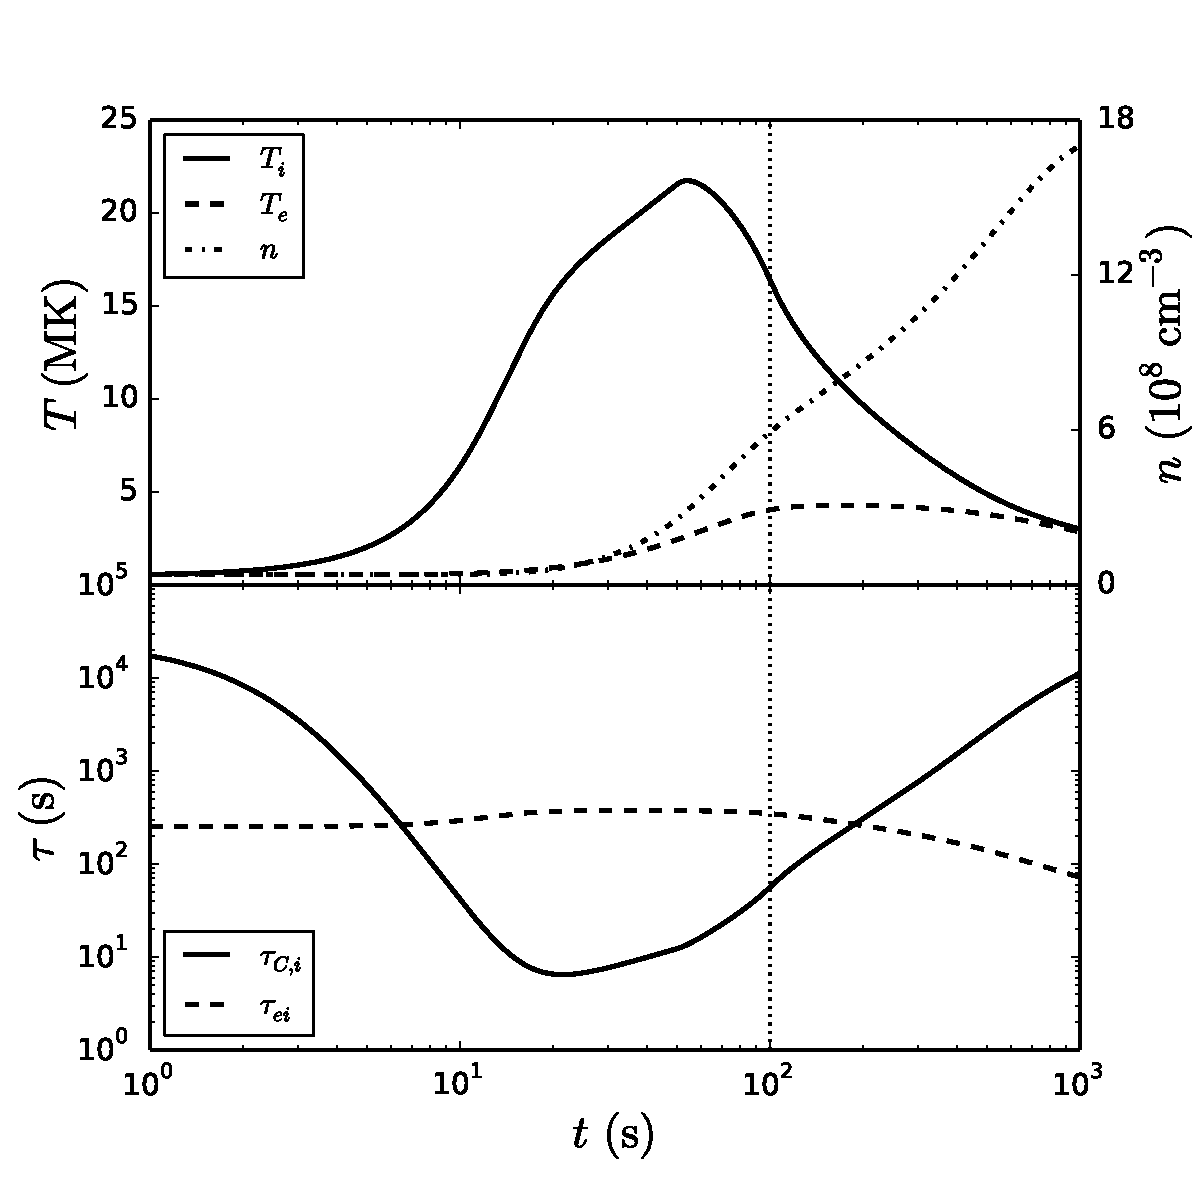
\includegraphics[width=\columnwidth]{figures/ion_ts_compare.pdf}
		\caption{Single triangular heating pulse with duration $\tau=100$ s and total energy $Q=10^{24}$ erg injected into only the ions in a loop of half-length $L=40$ Mm. \textbf{Top:} Ion temperature, electron temperature, and coronal number density. \textbf{Bottom:} Ion thermal conduction $(\tau_{C,i})$ and Coulomb collision $(\tau_{ei})$ timescales. The dotted black line at 100 s marks the end of the heating pulse.}
		\label{fig:ion_ts}
	\end{figure}
	%
	\par However, in the case of ion heating, in order for the emission measure to see the full range of temperatures resulting from the heating and conductive cooling by the ions, $\bar{T}_e=\bar{T}_i$ would have to hold for this entire phase. Instead, as the ions are impulsively heated, the electrons remain at a relatively low temperature, coupled only weakly to the ions because the loop has only just begun to fill. As the coronal density increases, the electrons come into equilibrium with the ions, but because thermal conduction is such an efficient cooling mechanism in the corona, the ions have now cooled far below the temperature to which they were initially heated. 
	\par This scenario is clearly illustrated by \autoref{fig:ion_ts}. In this test case, we have impulsively heated the ions with a triangular pulse lasting 100 s with total energy $10^{24}$ erg. In the top panel, we see that by the time the electrons come into equilibrium with the ions, the ions have cooled well below 10 MK and the loop has just begun to fill. Additionally, the bottom panel shows that during the period in which the ions are at their hottest temperatures, $\tau_{C,i}\ll\tau_{ei}$, where $\tau_{C,i}$ is the ion thermal conduction timescale. Thus, while they are being heated, the ions are giving up nearly all of their energy to thermal conduction before they reach equilibrium with the electrons.
	\par The result is a severely truncated hot emission measure distribution as seen in \autoref{fig:ion_em}. Additionally, this effect is exacerbated at long $T_N$. For short $T_N$, the heating is essentially steady, meaning that the loop has little to no time to drain or cool between heating events. This keeps the density at a roughly constant, near-equilibrium value which inhibits rapid heating to high temperatures and keeps the electrons and ions in equilibrium. However, for longer $T_N$, the loop is allowed to drain significantly between each pulse. Thus, at the start of each heating event, the density is low, allowing the species to very quickly evolve out of equilibrium. 
	%
	\par To address \autoref{itm:deriv} and \autoref{itm:histos}, we refer to our discussion in the introduction of \citetalias{cargill_hot_2016}. Using $\mathrm{EM}\sim n^2\tau_{cool}$ and assuming constant pressure (such that $n\propto T^{-1}$), in the free-streaming regime, $\mathrm{EM}\propto T^{-5/2}$; in the regime described by classical Spitzer conduction, $\mathrm{EM}\propto T^{-11/2}$. Thus, at high temperatures where the free-streaming limit is imposed to prevent runaway cooling by thermal conduction, we expect a much more shallow emission measure slope than at slightly lower temperatures where Spitzer conduction dominates.
	%
	\par Significant emission in the free-streaming regime is produced in the case of electron heating as evidenced by the hot shoulder in the emission measure curves of \autoref{fig:el_em}. The derivative in the lower-left panel also clearly shows the slope varying between roughly $-5.5$ and $-2.5$ as denoted by the two lower black dotted lines. Fitting a single slope to this entire range, we expect $2.5<b<5.5$ which is indeed the case as evidenced by the bottom-left panel of \autoref{fig:histos}. When characterizing such hot emission in the future, it may be more applicable to fit this emission with a double power-law in order to more properly account for these two distinct cooling regimes.
	%
	\par In the single-fluid case, the hot shoulder is not produced because there is not a significant amount of emission at temperatures where thermal conduction enters the free-streaming limit. This is likely for two reasons: (1) the heating is essentially equally partitioned between the electrons and ions, meaning less energy is directly injected into the electrons; (2) both species are helping to ``conduct away'' the excess energy through thermal conduction. Even if the free-streaming limit is reached in the single-fluid simulation, the density and amount of time spent in this regime are not significant enough to produce a signature (i.e. the hot shoulder) in the emission measure. In the case of ion heating, the emission measure never sees this temperature regime because the ions have cooled significantly by thermal conduction before they reach equilibrium with the electrons (as illustrated by \autoref{fig:ion_ts}). Thus, electron thermal conduction never comes close to the free-streaming limit because the electrons remain relatively cool.
	%
	\section{Conclusions}
	\label{sec:conclusions}
	%
	\par In this paper, we have used a modified two-fluid version of the popular EBTEL model to study the effect of preferentially heating the electrons or ions on the hot and cool emission measure slopes over a parameter space that includes the power-law index describing the distribution of event energies, $\alpha$, waiting time between successive heating events, $T_N$, and the scaling between the event energy and wait time, $\beta$. We have found that while there is little difference in the cool emission between the cases of electron and ion heating, when it comes to the hot emission, the emission measure curves of the electron-heated loops have an enhanced hot shoulder while the ion-heated loops show a truncated emission measure distribution on the hot side. This difference becomes more prominent as $T_N$ increases. We note that given such a distinction in the $\mathrm{EM}$ distribution between the cases of electron and ion heating, the difference could be potentially observationally diagnosable by instruments such as MaGIXS, the Focusing Optics X-ray Solar Imager (FOXSI) \citep{krucker_focusing_2011}, or other future missions with adequate spectroscopic resolution in the hard X-rays.
	\par Furthermore, by comparing these results with emission measure distributions obtained from the original single-fluid EBTEL model, we have found that heating only the electrons, because of the aforementioned hot shoulder due to flux limiting, leads to significantly more shallow hot emission measure slopes for equivalent values of $T_N$. Thus, using a single-fluid model to interpret observed hot emission measure distributions can potentially lead to a misdiagnosis of the heating frequency.
	%
	\par We note that in this study, we have constructed the most ideal emission measure curves by using the expression $\mathrm{EM}=n^2(2L)$; that is, we have not taken into account the many complications involved when computing emission measure distributions from observed spectral lines. For example, as we noted in \citetalias{cargill_hot_2016}, impulsive heating leads to non-equilibrium ionization and a consequently lower effective temperature, meaning that the emission does not see the hottest temperatures during the conductive cooling phase. Incorporating non-equilibrium ionization will thus narrow the emission measure distribution, leading to steeper emission measure slopes.
	%
	\par Additionally, using a more advanced forward modeling technique in the manner of \citet{bradshaw_what_2011} in which the limitations of both the instrument and the atomic data (as well as non-equilibrium ionization) are taken into account will likely further steepen the hot emission distribution. Thus, we stress that when interpreting observed hot emission in the context of simulation, two-fluid, non-equilibrium ionization, and instrument effects should all be properly taken into account in order to extract meaningful properties of the heating.
	%
	\section*{Acknowledgment}
	%
	All of the data analysis shown in this work was carried out using the IPython system for interactive scientific computing in Python as well as the NumPy and Scipy numerical and scientific Python libraries \citep{perez_ipython:_2007,van_der_walt_numpy_2011}. All plots were produced using the Matplotlib graphics environment \citep{hunter_matplotlib:_2007}.
	%begin appendix
	\appendix
	\section{}
	\label{appendix}
	%
	The modified two-fluid EBTEL equations are,
		\begin{align}
			\frac{d}{dt}\bar{p}_e &= \frac{\gamma - 1}{L}[\psi_{TR} + \psi_C -(\mathcal{R}_{TR} + \mathcal{R}_C)] + k_B\bar{n}\nu_{ei}(\bar{T}_i-\bar{T}_e) + (\gamma-1)\bar{E}_{H,e},\label{eq:press_e} \\[0.5em]
			%
			\frac{d}{dt}\bar{p}_i &= -\frac{\gamma - 1}{L}(\psi_{TR} + \psi_C) + k_B\bar{n}\nu_{ei}(\bar{T}_e-\bar{T}_i) + (\gamma-1)\bar{E}_{H,i},\label{eq:press_i} \\[0.5em]
			%
			\frac{d}{dt}\bar{n} &= \frac{c_2(\gamma-1)}{c_3\gamma Lk_B\bar{T}_e}(\psi_{TR} - F_{0,e}-\mathcal{R}_{TR}), 	\label{eq:density}
		\end{align}
		where 
		\begin{align}
			\psi_{TR} &= \frac{1}{1 + \xi}(F_{0,e} + \mathcal{R}_{TR} - \xi F_{0,i}), \label{eq:psi_tr}\\[0.5em]
			\psi_C  &= \bar{v}p_e^{(a)} - (p_ev)_0. \label{eq:psi_C}
		\end{align}
		Additionally, \autoref{eq:press_e}, \autoref{eq:press_i}, and \autoref{eq:density} are closed by the equations of state $p_e=k_BnT_e$ and $p_i=k_BnT_i$. 
		%
		\par The volumetric heating rates, $E_{H,e}$ and $E_{H,i}$, are the primary degrees of freedom in our model. In the case of electron (ion) heating, $E_{H,i}(E_{H,e})=0$. $\bar{p}_e,\bar{p}_i$ and $\bar{T}_e,\bar{T}_i$ are the spatially-averaged coronal electron and ion pressures and temperatures, respectively and $\bar{n}$ is the spatially-averaged coronal number density. $\mathcal{R}_C=\bar{n}^2\Lambda(T)$ is the volumetric coronal radiative loss rate, where $\Lambda(\bar{T})$ is the radiative loss function, and $\mathcal{R}_{TR}=c_1\mathcal{R}_C$ is the radiative loss rate in the transition region where the calculation of $c_1$ is described in \citet{cargill_enthalpy-based_2012}. Additionally, $F_{0,e},F_{0,i}$ are the electron and ion conductive fluxes as computed at the base of the loop, respectively, and are calculated using the classical Spitzer formula with a free-streaming limit imposed to prevent runaway cooling at low densities. The Coulomb collision frequency, $\nu_{ei}$, is given by,
		\begin{equation}
			\nu_{ei} = \frac{16\sqrt{\pi}}{3}\frac{e^4}{m_em_i}\left(\frac{2k_B\bar{T}_e}{m_e}\right)^{-3/2}\bar{n}\ln{\Lambda},
			\label{eq:col_freq}
		\end{equation}
		where $m_e,m_i$ are the electron and ion masses respectively and $\ln{\Lambda}$ is the Coulomb logarithm. Finally, $c_2=\bar{T}/T_a=0.6$, $c_3=T_0/T_a=0.9$, determined by static equilibrium, and $\xi=\bar{T}_e/\bar{T}_i$.
		%
		\par Note that in the limit that $\bar{T}_e=\bar{T}_i$ such that $\xi=1$, \autoref{eq:density} reduces to the single-fluid density equation of \citet{cargill_enthalpy-based_2012}. Additionally, \autoref{eq:press_e} and \autoref{eq:press_i} can be added together to recover the single-fluid pressure equation. As with the original EBTEL model, the modified two-fluid version has been successfully benchmarked against the HYDRAD hydrodynamic code.
	%
	%
	%Bibliography
	\bibliography{astrophys-abbrev.bib,references.bib}
	\bibliographystyle{apj}
	\clearpage
\end{document}